\chapter{Removing host dependency for optimization}
\label{cha:sys_fpgaonly}

In all the previous versions \texttt{MIDG2 FPGA}, \texttt{MIDG2 MPI FPGA} and the
first version with IO channels introduced in chapter \ref{cha:sys_arch},  the timestepping
loops which are dependent on the size of the meshes are present in the host.
Every iteration, the host uses the helper class \texttt{kernel\_group} method
\texttt{enqueue\_NDRange()} to enqueue the subgroup of the kernels to perform the
computation for that timestep and synchronize the kernel execution to sequentially
execute the kernels on non-shared elements followed by shared elements after the completion
of data transfers. This requires two host interactions per iteration, one to enqueue subgroup
\texttt{compute\_inner} and other to enqueue subgroup \texttt{compute\_halo} shown in Listing \ref{code:subgroups}.
The introduction of the IO channels for communication between the FPGAs allows the FPGAs
to communicate with each other without the need of host
for performing the communication.

As the host was not required anymore for communication, further optimization of the kernel structure
is done to remove the \texttt{host application} interaction completely. The change introduced is to implement the
the timestepping loops in the kernels and create a structure which only requires the \texttt{host application} to interact twice
per application invocation with the FPGA. Moving the timestepping loops to \texttt{kernels} additionally
required to implement a synchronization construct between the \texttt{kernels} to be able to process
the shared and non-shared data sequentially. This chapter introduces the modifications to \texttt{kernels}
and \texttt{host application} to achieve this \texttt{FPGA only} design. The chapter first
explains the \texttt{kernel} structures considered for implementing achieve a \texttt{FPGA only} system
along with the issues identified and their fixes. The chapter then discusses the final \texttt{FPGA only}
designs highlighting the optimization and changes from the previous versions in \texttt{kernel} and \texttt{host code}
In the last it discusses the issues identified during the optimization due to tool updates and changed kernel
structure to highlight the areas for improvements in the final design.

\section{Design considerations}

The first change required to remove the host dependency in the FPGA kernels was
to move the timestep loops to the \texttt{kernels} so that
they can iterate for the specified timesteps without needing the host to start them
every iteration. Implementing the timesteps in the kernels was easy. The timestep loops
are added at the top level above the existing code as shown in the pseudo code in \ref{code:timestep}.
To restrict the Intel OpenCL compiler from executing multiple iterations of the timestep iterations
and Runge-Kutta stages, the \texttt{\#pragma max\_concurrency 1} is added to the loops. This
Intel OpenCL directive, limits the concurrency of the loops to 1.
The complete modifications done to kernel codes is explained in section \ref{sec:final_struc}.
The actual timesteps are still computed in the \texttt{host application} and are passed as
parameter \texttt{NSteps} to kernels from the host. The actual value of the timestep is only known
after the kernels are enqueue and loop optimization are not possible. This change
additionally required to create a synchronization scheme in the kernels
to synchronize the communication kernels with the compute kernels
and to synchronize the iteration execution in each of the kernels.
This section presents the designs evaluated to identify the
best possible design for implementing the synchronization with
minimum overhead.

\begin{CppCode}[caption=Pseudo-code of kernel showing additional timestep loops added for
    creating FPGA only design, frame=tlrb, label=code:timestep, float]
__kernel void kernelName(__private int arg1,
                         __private int arg2,
                         __private int timesteps,
                         __global volatile float  *restrict buffer1,
                         __global volatile float  *restrict buffer2
                        )
{
    // Outer timestep loop
    #pragma max_concurrency 1
    for (int step = 0; step < timesteps; ++step)
    {
        // 5 RK steps
        #pragma max_concurrency 1
        for(int intrk = 0; intrk < 5; ++intrk)
        {
            // Old kernel code inside here
            // Process/Read/Write element
        }
    }
}
\end{CppCode}

\subsection{Synchronization using blocking Intel OpenCL channels}
\label{sec:sync_iochan}

The first design implemented utilizes the blocking Intel OpenCL channels
to communicate the synchronization events via the channels between the kernels.
As shown in Figure \ref{fig:iochan_kernstruc}, the existing pipeline
structure for the kernels is build up using the channels to separate the functionalities
for data access into separate input kernels (\texttt{S\_IN} and \texttt{V\_IN}
and computation kernels (\texttt{VOLUME} and \texttt{SURFACE}). The \texttt{RK}
as explained before is responsible for accumulating as well as writing the data into
the memory. This structure builds a pipeline where the data is fed at one end,
processed and then written into the memory at the other end of the pipeline every
iteration once for non-shared data and then for shared data after it is received
from other nodes.

In order to maintain the correct order of the processing in the kernels,
following synchronization needs to be achieved among the kernels.

\begin{enumerate}
    \item At the completion of data processing for non-shared elements, the input kernels should wait
    for the communication to complete
    \item The input kernels should wait for the last element to be processed and data written into the memory
    in the current iteration before moving into the next interaction
    \item The communication kernel should start communication at the start of every new iteration and wait
    until the processing is finished before starting the communication for the next iteration
\end{enumerate}

In the previous versions \texttt{MIDG2 FPGA}, \texttt{MIDG2 MPI FPGA} and \texttt{MIDG2 FPGA IO channels},
the \texttt{host application} performs these synchronizations. The host first starts the kernels
to process non-shared data along with communication kernels which execute parallely. The hosts waits for
kernels to finish the processing the non-shared elements using the \texttt{waitforcompletion()} method and
for the MPI to finish communication using \texttt{MPI\_waitall()} API before starting
kernels again to process shared elements. This sequence of operations is shown in Figure
\ref{fig:sequence_comp} (a).

The first iteration of this design used 5 blocking channels to synchronize the above mentioned
events as shown in Figure \ref{fig:channelsync_kernstruc}.
The arrows in the Figure denote the read/write dependency of the kernel on the channels.
Kernel from where the arrow starts is responsible for writing the data into the channel
and the end kernel reads this data. The synchronization is achieved by the blocking
nature of the channels. For example, to synchronize an event between two kernels,
\texttt{kernel1} and \texttt{kernel2}, they are connected with a channel named \texttt{syncChannel}.
Whenever \texttt{kernel1} should wait for an event from the \texttt{kernel2},
\texttt{kernel1} invokes a blocking read using \texttt{read\_channel\_intel(syncChannel)} on the
\texttt{syncChannel} between the kernels which makes
\texttt{kernel1} block on the channel read. Once the event happens \texttt{kernel2} writes a token in the channel
which unblocks \texttt{kernel1}. As the channel are uni-directional, the blocking nature is suited
to achieve the synchronization required in the MIDG2 kernels.

\begin{figure}[ht]%
    \centering
    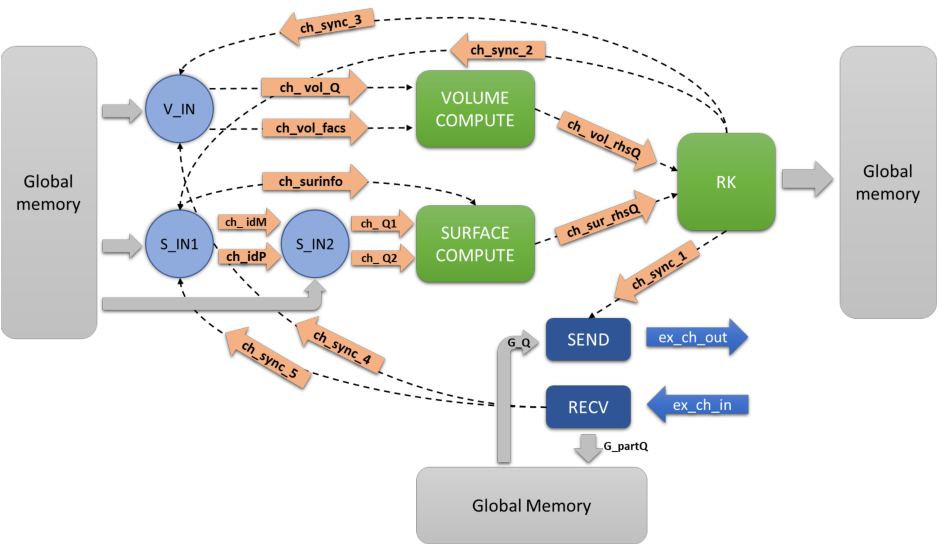
\includegraphics[width=1.0\textwidth]{images/channelssync_kernstruc}
    \caption{Kernel structure for FPGA only design utilizing 5 blocking channels for synchronization}
    \label{fig:channelsync_kernstruc}
\end{figure}

In the design, \texttt{ch\_sync\_1} between \texttt{RK} kernel and the send kernel is to synchronize
the start of communication at the beginning of each iteration. \texttt{ch\_sync\_2} and
\texttt{ch\_sync\_3} is used to synchronize the completion of writing last element into
the memory to start of reading the elements in the next iteration by the input kernels.
\texttt{ch\_sync\_4} and \texttt{ch\_sync\_5} is used to synchronize the completion
of communication from the \texttt{recv} kernels. Though the required sequence of operation
was achieved with the channels and speed up was noticed, the design didn't produce correct
results which was identified due to large deviation in the analytical and the computed
nodal error values. After further analysis of the design it was noticed that the
\acl{LSU} in input kernels used cached access for \texttt{g\_Q\_ping} and \texttt{g\_Q\_pong}
buffer reads which could be a problem with the updated design. As the buffer is updated by the
\texttt{RK} kernel and the kernels are supposed to switch the buffers in each iteration, cached reads
could lead to processing of stale values resulting in wrong field computation. To eliminate
the cache for the memories, the buffer parameters were marked as \texttt{volatile} which allows
to remove cached access \cite{noauthor_intel_2019,section 9.4} to ensure correct sequence of
reads and writes. This allowed removal
of the cache for all the read \texttt{LSU} but still deviation in the nodal errors were
present and further analysis was done to identify the cause.

\subsection*{Addition of latency}
\label{sec:add_latency}

Another probable issue with the design was with the difference in latency of memory operation
and channel communication. As the channels are implemented as FIFOs in the hardware
using registers or BRAMs, the latency of the channels is much smaller than that of a memory
operation. This would cause the input kernels to access non-updated memory after receiving the
event over the channels. As shown in the Figure \ref{fig:memchan_latency} (a), due to higher latency
of the memory to handle the write request which is not visible in the kernel, an overlapped
read is possible while using channels for synchronization.
\begin{figure}[h]
	\centering\small
	\begin{tabular}{c|c}
    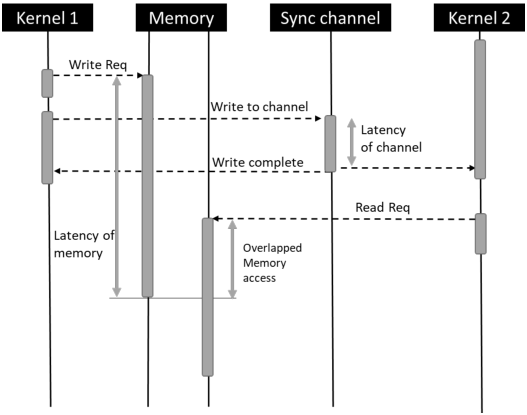
\includegraphics[width=0.45\textwidth]{images/memchan_latency} & 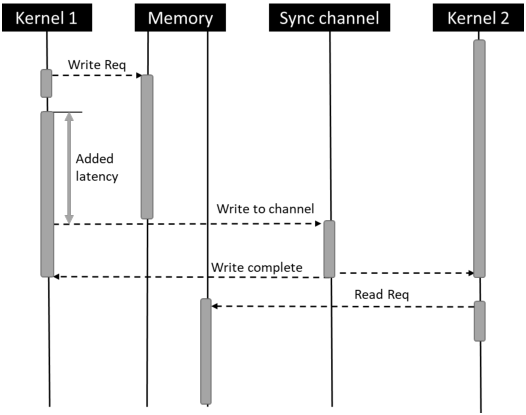
\includegraphics[width=0.45\textwidth]{images/resolved_latency}\\
    (a) & (b)
	\end{tabular}
    \caption{Sequence of operation between kernels to synchronize memory
    access with channels. (a) Shows the latency differences for memory and
    channel causing overlapped memory access. (b) Shows the sequence with
    added latency which avoids the overlap}
	\label{fig:memchan_latency}
\end{figure}
% \begin{figure}[ht]%
%     \centering
%     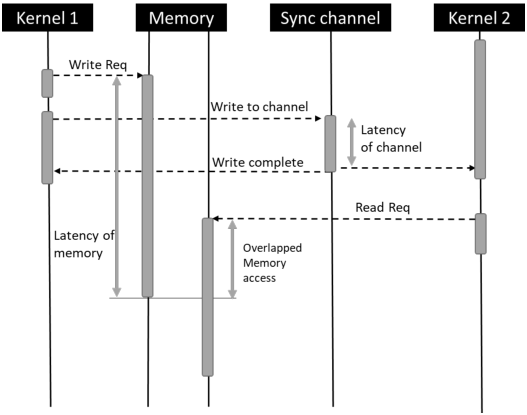
\includegraphics[width=0.6\textwidth]{images/memchan_latency}
%     \caption{Sequence of operation between kernels using memory and channels showing
%     the latency differences for memory and channel and its effect while using
%     for synchronization}
%     \label{fig:memchan_latency}
% \end{figure}

As there is no concrete information available for the target board to estimate
the exact latency for the memory and no method to block on the
completion of the memory operation, it was not possible to fix this issue with
a deterministic solution. Alternatively, a latency could be introduced after the
invocation of last element write to ensure that the write memory operation complete before
the read is invoked in the next iteration. As addition of latency in the OpenCL
kernels in not trivial due to lack of standard APIs to add wait or sleep in the kernel,
a latency logic was created using loops. A loop with an \ac{II}
of 1 can be used to create a latency for a desired amount of time by varying the
loopcount. This is achieved by placing a channel write instruction in a loop
as shown in the Listing \ref{code:latency}. The loop is pipelined with a II=1
is generated which is executed for \texttt{waitCount} iterations before writing
the \texttt{token} into the channel. The \texttt{waitCount} is configured as a kernel
parameter to vary the latency as per requirement as there is no easy deterministic way to measure
the exact latency required. The latency in seconds added can be calculated using the
frequency of the synthesized design using the formula

$$ latency(in seconds) = \frac{waitCount}{Frequency(Hz)} $$

\begin{CppCode}[caption=Loop structure used to add latency in the kernels, frame=tlrb, label=code:latency, float]
for(int time = 0; time < waitCount; ++time)
{
    if (time == waitCount - 1)
    {
        write_channel_intel(channel, token);
    }
}
\end{CppCode}

Using this loop structure, latency was introduced
in \texttt{RK} and \texttt{recv} kernels placing the channels \texttt{ch\_sync\_1},
\texttt{ch\_sync\_2} and \texttt{ch\_sync\_3} in a wait loop in the \texttt{RK} kernel and \texttt{ch\_sync\_4}
and \texttt{ch\_sync\_5} in the another wait loop in \texttt{recv} kernel to avoid
overlapped access of \texttt{g\_Q} and \texttt{g\_partQ} buffers. Introduction
of latency changes the sequence of operations as shown in the Figure \ref{fig:memchan_latency} (b)
which shows no overlapping in the memory requests due to latency.

% \begin{figure}[ht]%
%     \centering
%     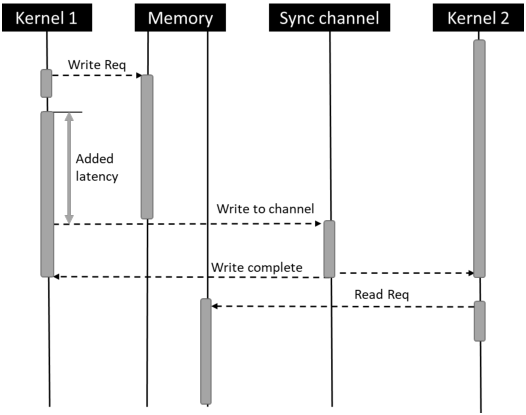
\includegraphics[width=0.6\textwidth]{images/resolved_latency}
%     \caption{Sequence of operation with added latency to avoid overlapped
%     memory access}
%     \label{fig:resolved_latency}
% \end{figure}

\subsection*{Removing channels \texttt{ch\_sync\_2} and \texttt{ch\_sync\_3}}

Another issue reported by the Intel OpenCL compiler as warning was the formation of looping
structure within the kernels due to use of the channels for synchronization.
Addition of the \texttt{ch\_sync\_2} between RK and \texttt{S\_IN1} kernel created
a loop of the kernels \texttt{S\_IN1} -> \texttt{S\_IN2} -> \texttt{SURFACE} -> \texttt{RK} -> \texttt{S\_IN1}.
Similarly, addition of \texttt{ch\_sync\_3} created a loop \texttt{V\_IN} -> \texttt{VOLUME} -> \texttt{RK} -> \texttt{V\_IN}.
Creation of these loops avoided Intel OpenCL compiler to optimize the channel depths
which caused increased latency of the pipeline and decreased performance.

After further analysis and tests with different kernel structure, it was identified that
after addition of the \texttt{volatile} keyword for the buffers as explained in \ref{sec:sync_iochan},
an implicit synchronization of the memory operations is created between \texttt{kernels} and the removal of channels \texttt{ch\_sync\_2} and
\texttt{ch\_sync\_3} does not affect overall functionalities of the design in terms of speed
and correctness. Due to this, it was decided to remove these channels which allowed the
compiler to optimize the channel depth and improve performance.

\subsection{Synchronization using locks with atomic memory operations}

Apart from using channels for synchronization another possibility to achieve
the desired behavior was by using atomic memory operations in the kernels
to create a locking/unlocking structure for synchronization. Intel
OpenCL FPGA SDK supports the standard OpenCL \textit{Atomic Functions for 32-bit Integers}
listed in \ref{code:atomic_func}.

\begin{CppCode}[caption=Interger versions of the atomic operations supported by Intel
    OpenCL FPGA SDK, frame=tlrb, label=code:atomic_func, float]
int atomic_add(volatile __global int *p, int val)
int atomic_sub(volatile __global int *p, int val)
int atomic_xchg(volatile __global int *p, int val)
int atomic_inc(volatile __global int *p)
int atomic_dec(volatile __global int *p)
int atomic_cmpxchg(volatile __global int *p, int cmp, int val)
int atomic_min(volatile __global int *p, int val)
int atomic_max(volatile __global int *p, int val)
int atomic_and(volatile __global int *p, int val)
int atomic_or(volatile __global int *p, int val)
int atomic_xor(volatile __global int *p, int val)
\end{CppCode}

The atomic operations were used to create a similar synchronization effect as done with the channels.
\texttt{atomic\_cmpxchg} and \texttt{atomic\_xchg} functions are used to check and update the
memory as shown in code listed in \ref{code:atomic_impl}. Four memory locations in the global memory are used
for four synchronization behavior. The first and second location is to synchronize the access to \text{g\_Q} memory
between \texttt{RK-VOLUME} and \texttt{RK-SURFACE} pairs respectively. \texttt{VOLUME} and \texttt{SURFACE} kernel wait for the \texttt{RK} kernel
at start of every iteration to clear the memory to mark the start of new iteration. Immediately
after clearing the memories, both write a specific token value to denote start.
The third and fourth memory locations are to synchronize the start of communication and
completion of communication. Send kernel waits for the memory location to be cleared
by the volume and \texttt{SURFACE} kernel at the start of every new iteration to start the communication.
The same memory location is checked by volume and \texttt{SURFACE} kernel after completion of processing
the non-shared elements to have a specific token value written by the recv kernel after the completion
of communication. This creates the synchronization between the start of communication to end of communication
for processing the shared data.

\begin{CppCode}[caption=Synchronization Implementation with atomic functions, frame=tlrb, label=code:atomic_impl, float]
#pragma max_concurrency 1
for (int step = 0; step < timesteps; ++step)
{
    #pragma max_concurrency 1
    for(int intrk = 0; intrk < 5; ++intrk)
    {
        // Wait for memory 1 to be cleared
        while (atomic_cmpxchg(&lock[1], 0, 0xFB) == 0xFB);

        // Clear memory 3
        atomic_xchg(&lock[3], 0);
    }
}
\end{CppCode}

As with channels, this design also had several similar issues. The use of atomic APIs are very expensive and
reduce the clock frequency and overall performance of the design diminishing any benefit from the improved
structure. Also like with channels, the memory latency resulted in incorrect results and required additional
latency to be include. As the design was not good in terms of performance further analysis to fix the issues
identified were not carried out due to time constraints

\section{Final optimized Design}
\label{sec:final_struc}

The final design which is used for the evaluation and highlighting the benefits of the design includes
options selected after multiple iterations of variations in the design in terms of kernel
structure for synchronization, loop structure, variation in sequence of kernels and variation
of the memory channel assignment to get the most optimized design as a whole. This section
will present in detail individual aspect of the final design bringing the changes together
in the kernel as well as in the host code.

\subsection{Kernel Structure}

The final design with the selected optimization to maximize the performance of the kernel and achieve
higher speed up was created using the design introduced in section \ref{sec:sync_iochan}.
The final optimized design is shown in Figure \ref{fig:fpgaonly_kernstruc}.

\begin{figure}[ht]%
    \centering
    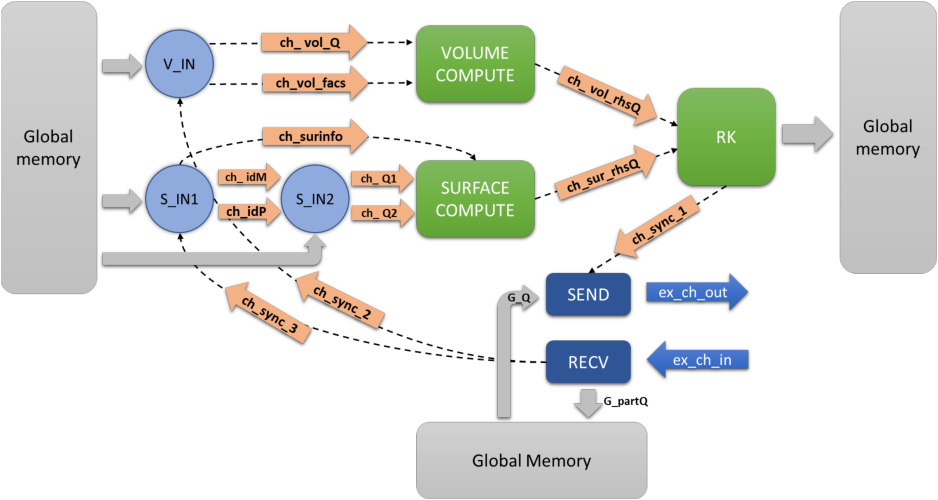
\includegraphics[width=1.0\textwidth]{images/fpgaonly_kernstruc}
    \caption{Kernel structure of the optimized FPGA only design}
    \label{fig:fpgaonly_kernstruc}
\end{figure}

The kernels independent of host executes for \texttt{Nsteps} timestep iterations.
In each timestep iteration 5 RK stages are executed. Within each RK stage, \texttt{K}
elements are read processed and written back to the memory. The kernels form a pipeline
where the k\textsuperscript{th} element and other coefficients required are read by the
input kernels from the global memory and forwarded to the compute kernels by channels.
The compute kernels process the element to compute the right-hand side field values and
forwards it to \texttt{RK} kernel. There the field values are accumulated and stored in global memory.
In between the shared data is communicated and used for computation. Due to the long pipeline,
multiple elements are processed simultaneously in different stages of the pipeline giving
higher throughput and performance.

The changes included in the final kernel structure are minor changes done to improve the performance
and fix issues identified during testing of the different variations of the FPGA only implementation.
Following points consolidate all the changes done to base design to achieve the final optimized
design.

\subsubsection*{Loop coalescing}

The major change from the base design introduced in section \ref{sec:midg2_mpi} to the
optimized design is the introduction of the timestep loops in the kernels as shown in
code \ref{code:timestep}. The introduction of these loops removed the dependency of the kernels
on the host code for the timestepping but at the same time created the problem of increased
nested loop depth. The increased nested loop depth is not ideal as it makes it harder
for the Intel OpenCL compilers to optimize the loop pipelining. Another problem is
increase in the resource utilization as additional 'control hardware' resources are
required to handle each of the nested loops. To reduce the effects of this necessary
change, in the final design, the top two levels of the nested loops were coalesced
using the pragma \texttt{loop\_coalesce} as shown in the kernel pseudo-code in \ref{code:coalesce}.
Use of \texttt{loop\_coalesce} does not change the behavior of the actual loops instead
only decreases the hardware resources required to handle the loops.
\begin{CppCode}[caption=Loop coalescing used for additional timestep loops in FPGA only design, frame=tlrb, label=code:coalesce, float]
__kernel void kernelName(__private int arg1,
                            __private int K,
                            __private int timesteps,
                            __global volatile float  *restrict buffer1,
                            __global volatile float  *restrict buffer2
                        )
{
    // Outer timestep loop
    #pragma loop_coalesce 2
    for (int step = 0; step < timesteps; ++step)
    {
        // 5 RK steps
        for(int intrk = 0; intrk < 5; ++intrk)
        {
            for (int k=0; k < K; k++)
            {
                // Old kernel code inside here
                // Read/Process//Write k/+\textsuperscript{th}+/ element
            }
        }
    }
}
\end{CppCode}

\subsubsection*{Volatile memories and Buffer management}

As it was identified during the analysis of the design with IO channels used
for synchronization \label{sec:sync_iochan} that the caching for memory was resulting
in wrong results. The Memory buffers \texttt{g\_Q1\_ping}, \texttt{g\_Q1\_pong}, \texttt{g\_Q2\_ping},
\texttt{g\_Q2\_pong} and \texttt{g\_partQ} are marked as volatile memory to avoid
caching of the read \ac{LSU}s. Along with the use of volatile memory, a buffer management
scheme explained in the Buffer Management section in the Intel FPGA SDK for OpenCL Pro Edition: Programming Guide
\footnote{\url{https://www.intel.com/content/www/us/en/programmable/documentation/mwh1391807965224.html}}
was implemented to complement the synchronization via channels. The \texttt{mem\_fence}
with \texttt{CLK\_GLOBAL\_MEM\_FENCE} and \texttt{CLK\_CHANNEL\_MEM\_FENCE} flags were introduced
after the buffer writes in the \texttt{RK} and \texttt{recv} kernels as explained in the document.

\subsubsection*{Communication Channels}

The final design uses only three channels for synchronization as shown in the kernel
structure in Figure \ref{fig:fpgaonly_kernstruc}. The first channel is used between RK and
\texttt{send} kernel to synchronize the start of the communication with the end of last iteration.
The latency loop structure is used in the RK kernel which ensures that the \texttt{send}
kernel reads the correct values from the \texttt{g\_Q} buffer. Channels 2 and 3 connect from
\texttt{recv} to \texttt{VOLUME} and \texttt{SURFACE} kernels to synchronize the end of the
communication with the start of processing the shared elements. These channels writes are also within
latency loop to add a delay for the read of the \texttt{g\_partQ} buffer in \texttt{SURFACE} kernel.

\subsubsection*{Moving RK coefficients into kernel}
Moving timestep loops into the kernels allowed an additional minor optimization in the design.
The Low storage Runge-Kutta coefficients used for the accumulating the right-hand side field values from
\texttt{VOLUME} and \texttt{SURFACE} kernels were passed from the host application in each time step
iteration. This was done from host as for each of the 5 Runge-Kutta stages a different coefficient is used
and since the timestep and RK stage control was done in host application, the host selected the respective
timestep-RK-stage coefficient and updated in the kernel private memory. Accessing the float coefficient
add a small latency in each iteration of the execution and as the timestep loops were shifted to the kernels,
the coefficients which are in total 10 float values are now stored in the kernel as constant arrays as shown
in the code Listing \ref{code:rkcoeff}. This removes an additional memory access required to select the
coefficient and improves the memory bandwidth and overall kernel performance.

\begin{CppCode}[caption=Use of Runge-Kutta coefficients inside the \texttt{RK} kernel, frame=tlrb, label=code:rkcoeff, float]
__kernel void rkkernel(..Args..)
{
    const float rk4a[5] = {Vs1,Vs2,Vs3,Vs4,Vs5};
    const float rk4b[5] = {Vs1,Vs2,Vs3,Vs4,Vs5};
    // Outer timestep loop
    #pragma loop_coalesce 2
    for (int step = 0; step < timesteps; ++step)
    {
        // 5 RK steps
        for(int intrk = 0; intrk < 5; ++intrk)
        {
            // Select the RK-coefficient for the stage
            float l_fa = rk4a[intrk];
            float l_fb = rk4b[intrk];

            // Old kernel code inside here
            // Process/Read/Write element
        }
    }
}
\end{CppCode}

\subsubsection*{Buffer Aliasing}

The change in the structure of the kernels due to introduction of the timestep loops
required to move the buffer switching for the duplicated buffers \texttt{g\_Q\_ping} and
\texttt{g\_Q\_pong} inside the kernels since host has no interactions with FPGA anymore
during the timesteps. The input kernels and \texttt{RK} kernels receive both buffers as parameters
and implement a switching logic as shown in the line number 17 and 18 in Listing \ref{code:buf_switch}.
The switching is done to switch the input buffer and the output buffer after every iteration
which allows parallel execution of the all the kernels for computation.
\begin{CppCode}[caption=Buffer switching for FPGA only design within the kernel, frame=tlrb, label=code:buf_switch, float]
__kernel void kernelName(__private int K,  __private int arg2,  __private int timesteps,
                        __global volatile float  *restrict g_Q_ping,
                        __global volatile float  *restrict g_Q_pong
                        )
{
    // Outer timestep loop
    #pragma loop_coalesce 2
    for (int step = 0; step < timesteps; ++step)
    {
        // 5 RK steps
        for(int intrk = 0; intrk < 5; ++intrk)
        {
            // compute timestep
            int stepCount = step*5 + intrk;

            // switch the buffer: Ping in EVEN step, Pong in ODD
            __global volatile float *restrict g_Q_in = (stepCount%2 == 0)? g_Q_ping:g_Q_pong;
            __global volatile float *restrict g_Q_out = (stepCount%2 == 0)? g_Q_pong:g_Q_ping;

            // Iterate over the elements
            for (int k = 0; k < K k++)
            {
                float somevalue = g_Q_in[k];
                ...
                somevalue = somevalue + anothervalue;
                ...
                g_Q_out = someothervalue; // Creates Write-ACK LSU
            }
        }
    }
}
\end{CppCode}

The buffer switching using the above logic works correctly though resulted in false memory
dependencies identifications in \texttt{RK} kernel by the compiler. As \texttt{g\_Q\_in} and
\texttt{g\_Q\_out} are assigned the same buffers alternatively which compiler is unable to
identify from the above structure and reports memory dependencies between the read and write
memory operations which follow one another as shown in the pseudo-code (line numbers 23-27) \ref{code:buf_switch}.
Due to the identified memory dependencies, the compiler adds the write-ack LSU for the writing
operations which have higher latency and ensure that write operation is completed before
any other operation on the same buffer is started. This is a false memory dependency which
results due to inability of the compiler to identify the specified switching behavior.
In order to solve this problem which resulted in decreased performance, memory aliasing
is done for \texttt{g\_Q\_ping} and \texttt{g\_Q\_pong} memories similar to one done for the
\texttt{g\_partQ} memory. For aliasing, additional duplicate memory buffer parameters are
assigned to kernel and used to assign the double buffers as shown in the pseudo-code \ref{code:resolve_alias}.
In the \texttt{host application} the same OpenCL memory buffer is assigned to both the parameters instead of creating
additional memories which is not required. This fools the compiler to accept them as two different
memories and avoid write-ack LSU.
\begin{CppCode}[caption=Aliasing of the \texttt{g\_Q\_xx} buffer to avoid memory dependencies
    identified by the Intel OpenCL compiler, frame=tlrb, label=code:resolve_alias, float]
__kernel void kernelName(__private int K,  __private int arg2, __private int timesteps,
                        __global volatile float  *restrict g_Q_ping,
                        __global volatile float  *restrict g_Q_pong,
                        __global volatile float  *restrict g_Q_ping_2,
                        __global volatile float  *restrict g_Q_pong_2
                        )
{
.....
    // switch the buffer: Ping in EVEN step, Pong in ODD
    __global volatile float *restrict g_Q_in = (stepCount%2 == 0)? g_Q_ping:g_Q_pong;
    __global volatile float *restrict g_Q_out = (stepCount%2 == 0)? g_Q_pong_2:g_Q_ping_2;
.....
}
\end{CppCode}

Similar approach was used with \texttt{g\_resQ} memory also to
avoid the same problem by aliasing the buffer into \texttt{g\_resQ\_in} and \texttt{g\_resQ\_out}.
As the texttt{g\_resQ} write for a element is always scheduled after the read for that element in the
\texttt{RK} kernel as shown in the kernel execution sequence in Figure \ref{fig:resQSeq},
the operations have no dependencies and can be aliased.
\begin{figure}[ht]%
    \centering
    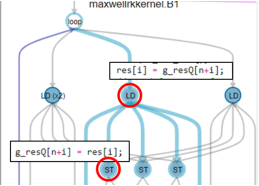
\includegraphics[width=0.6\textwidth]{images/resgSeq}
    \caption{\texttt{RK} kernel execution sequence showing read of \texttt{g\_resQ} followed by
    write}
    \label{fig:resQSeq}
\end{figure}

\subsection{Host code updates}
\label{sec:hostcodeupdate}

Addition of the FPGA only design required reworking of the host code in order to
support all the designs variants with a single host code for performing the evaluation.
Apart from the multi design support changes there are also other minor changes done in the code necessary
to initialize the memories for the kernel buffers at aligned boundaries and some other
changes. This section will discuss the changes in detail to give an understanding
to the reader.

\subsubsection*{Restructuring of the configuration module}

The major change in the host code is done to the module structure of
the code responsible for handling the the OpenCL platform initialization,
configuration and execution. With the addition of FPGA only design,
three variants of the kernels are available viz. \texttt{MIDG2 MPI FPGA} (SingleFPGA),
FPGA-to-FPGA communication using IO channels with host synchronization (MultiWithHost)
and FPGA only design (MultiFPGAOnly). Initially different versions of the same
configuration code were used by including or excluding design specific changes
using preprocessor directives or by selecting different files for compilation.
This intermediate solution allows the host code to support only single design
and requires modifications and recompilation of the code every time to use other
design. Additionally, the designs with IO channel communication also have two variants
with minor configuration changes which also increase the complexity of the host code.

To build a simpler and understandable host code which is able to support all the three
designs in a single binary, the host code is restructured by introducing hierarchical
structure for the OpenCL handling part. The structure of the modified host code is
shown in Figure \ref{fig:host_appstruc}. The restructuring does not modify the existing interface to the
OpenCL configuration routine instead splits the configuration module into device
specific and design specific configuration modules. The \texttt{BuildRunCLDevice}
provides the generic interface for OpenCL device configuration and execution.
The design specific run modules \texttt{RunSingleFpga}, \texttt{RunMultiWithHost}
and \texttt{RunMultiFpgaOnly} performs the design specific memory configuration
and setup to run the specific kernels on the device. The design specific run module
is configured at the run time by providing the command line parameter
\texttt{-d <DESIGN>} which allows a single host code to handle all the designs
without requirement for a recompilation.
\begin{figure}[ht]%
    \centering
    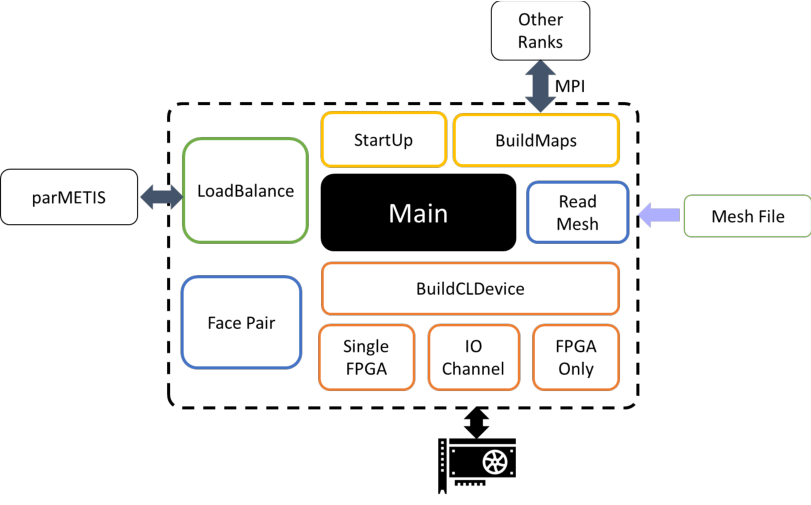
\includegraphics[width=0.8\textwidth]{images/host_appstruc}
    \caption{Module structure of the the host application after restructuring showing
    three separate sub-modules to handle OpenCL device configuration}
    \label{fig:host_appstruc}
\end{figure}

To achieve this restructuring additional structures were included which allows to
group the variables into functionality based groups. A important structure
to hold the function pointers to design specific routines is created
as shown in Listing \ref{code:interface_func}. This structure is initialized
with the design specific routines to handle device functionalities which
include creation of OpenCL buffers, Initialization of kernel arguments,
writing data into the device global memory and design specific cleanup.
Each of the design specific modules initializes individual structures
with the specific routines. The top level \texttt{BuildRunCLDevice} requests
a pointer to this structure at the runtime using the \texttt{XXXX\_getDeviceIntfHandlers()}
function. The handlers for only the selected design is requested and used to configure the
FPGA with the selected design kernels.
\begin{CppCode}[caption=Structure to hold the design specific interface function pointers
    and initialization example, frame=tlrb, label=code:interface_func, float]
// Structure to hold the interface functions
typedef struct
{
    void (*fnInitKernelArgs)(tClObjs* clObjs, Mesh* mesh, tChannelInfo* channelInfo,
                             char* kernelConfig);
    void (*fnFreeKernelMem)(tClObjs* clObjs);
    cl_int (*fnCreateBuffers)(tClObjs* clObjs);
    cl_int (*fnWriteToBuffers)(tClObjs clObjs, tKernelInitParams params);
    void (*fnRunKernel)(Mesh *mesh, tKernelRunParams* runparams, tProfileInfo* profileInfo,
                        tKernelInfo kernelinfo, tClObjs* clObjs);
    int (*fnGetKernelData)(tClObjs clObjs, float* c_resQ, float* c_Q,
                           tKernelInitParams params, Mesh *mesh);
} tclIntfHandlers;

// Initialization example in the sub-module
static tclIntfHandlers intfHandlers =
{
    initKernelArgs,
    FreeKernelMem,
    createBuffers,
    writeToBuffers,
    runKernel,
    getKernelData
};

// Access function to get the pointer to the interface
// handlers structure variable
tclIntfHandlers* XXXX_getDeviceIntfHandlers(void)
{
    return &intfHandlers;
}
\end{CppCode}

This structure allows the host application to request the design specific handlers at the
runtime and support different designs in one binary. The modifications were useful in testing
and evaluation of the designs.

\subsubsection*{Utilize all Memory channels of BittWare 520N}

The BittWare 520N boards using Intel Stratix 10 FPGA provides 4 external memory channels
to access the global memory. Each of the
4 external memory channels can be used parallely by the kernels to read and write data
into the global memory. Placing OpenCL buffers into different memory channels can
improve memory bandwidth and overall performance of the kernels by reducing the stalls
for simultaneous memory requests and reducing the latency of memory reads/writes.
A OpenCL buffer can be configured in the host code to be placed in a specific channel
by using the \texttt{CL\_CHANNEL\_X\_INTELFPGA} flag during the creation of the memory
as shown in the code below. \texttt{X} should be replaced with the channel number in which
the buffer has to be placed. For Stratix 10 \texttt{X} can be from 1 to 4 as it supports 4 channels.
Earlier Arria 10 boards supported only two channels.
\begin{CppCode}
cl_mem clMem;
clMem = clCreateBuffer(context, (CL_MEM_HETEROGENEOUS_INTELFPGA | CL_CHANNEL_1_INTELFPGA), size, NULL, &ret);
checkError(ret, "Failed to create buffer");
\end{CppCode}

The MPI implementation was designed and optimized for the BittWare 385A FPGA Accelerator Card which has a
Intel Arria 10 GX FPGA. As the board supported only two channels, the host code used only two channels
to distribute the memory buffers in the most optimal scheme. As there were additional two channels
available on the BittWare 520N board, the host code was updated for the base design to utilize
all the 4 channels. The modifications improved the bandwidth performance of the base design
as well as the overall execution time by small factors. The memory channel scheme
for the base design was not suitable for the final design since all the kernels execute
parallely as well as there are some memory buffers not used any more in the final design.
The profile information of the final kernel design was used to come up with a
different channel assignment scheme which distributed the memory load to all the
four channels equally. The updated scheme uses channel 4 for \texttt{Q2 Pong} buffer
as it was noticed to have stalls of upto 60\% to 70\% on writes to the buffer in the \texttt{RK}
kernel. Stalls in the \texttt{RK} kernel are propagated over the complete pipeline of the kernels
as all are connected via channels reducing the occupancy. Updating the channel reduced
the memory stalls to 7\% to 10\% and improve the memory bandwidths and performance
of the whole pipeline. Another change was to use channel 3 for the \texttt{g\_resQ}
buffer instead of channel 2. As channel 3 is highly utilized by other memory buffers as well
and channel 2 is will only be occupied in the even or odd iterations due to buffer switching,
this change reduces the stalls for the \texttt{g\_resQ} buffer read and write.
The final channel assignment used for base \texttt{MIDG2 MPI FPGA} design, the \texttt{MIDG2 FPGA IO channels} and
\texttt{FPGA only} design is shown in table \ref{tab:channel_assign} and the definitions of the symbols used for size computation as below.
\begin{table}[ht]
    \begin{center}
        \caption{Updated memory channel assignment for the buffers in \texttt{MIDG2 MPI FPGA}, the \texttt{MIDG2 FPGA IO channels} and
        \texttt{FPGA only} design}
        \label{tab:channel_assign}
        \begin{tabular}{|l|l|C{3cm}|C{3.4cm}|} %
          \hline
          \textbf{Buffer} & \textbf{Size} & \textbf{MPI FPGA} & \textbf{FPGA ONLY/IO CHANNEL}\\
          \hline
          Q1 Ping &   & 1 & 1 \\
          \cline{1-1} \cline{3-4}
          Q1 Pong &  & 1 & 1 \\
          \cline{1-1} \cline{3-4}
          Q2 Ping &   & 2 & 2 \\
          \cline{1-1} \cline{3-4}
          Q2 Pong & \texttt{K* BSIZE * pNfields}  & 2 & 4 \\
          \cline{1-1} \cline{3-4}
          surrhsQ &   & 3 & - \\
          \cline{1-1} \cline{3-4}
          volrhsQ & & 4 & - \\
          \cline{1-1} \cline{3-4}
          ResQ & & 3 & 2 \\
          \hline
          Mappping Info & \texttt{K* Nfp * NFaces * 2}  & 3 & 3 \\
          \hline
          Surface Info & \texttt{K* Nfp * NFaces * 5} & 3 & 3 \\
          \hline
          partQ & \texttt{Ntotalout} & 4 & 4 \\
          \hline
          parMapOut & \texttt{Ntotalout}  & 3 & 3 \\
          \hline
          vgeo & \texttt{12 * K}  & 3 & 3 \\
          \hline
        \end{tabular}
    \end{center}
 \end{table}
 \begin{verbatim}
    N = Order of the DG nodes
    Np = ((N + 1) * (N+2) * (N+3)/6)
    K = Number of elements
    BSIZE = Np
    Nfp = Number of DG nodes on each face of tetrahedral = (N+1) * (N+2)/2
    Ntotalout = Number of shared fields
\end{verbatim}

\subsubsection*{Alignment of the memory}

The external channels support only 256 bits transfers. The first version
using the IO channels for within the node topology used all the 256 bits
to transfer data. This required aligning the partial memory buffer
at 32 byte boundary to receive the data correctly. As the \texttt{partial\_send}
kernel requires to read the data from the \texttt{g\_Q} buffer from random
locations in as a group of 6 floats (24 bytes), use of 32 byte data transfers
was not efficient for the non-aligned memory access. To avoid this, the transfers
were modified to send 24 bytes of actual data and pad the rest 8 bytes with 0s.
This allowed to coalesce the 24 byte reads and improve the performance.

The similar approach was initially used for \texttt{fully connected} topology where
24 bytes of data on all 4 channels were transferred simultaneously. The send had
no issues with this structure but as explained in section \ref{sec:struc_iochan},
the writes to \texttt{g\_partQ} buffer were identified as dependent leading
to serial receives on the external channels and aliasing was used to solve this.
The aliasing done requires the individual partitions of the shared memory to be aligned
on a 64 byte as well as on a 24 byte aligned boundary. The 64 byte alignment is required
to ensure that the parallel writes to each of the aliased buffer do not overlap due to
cache line sharing. The cache is aligned on a 64 byte boundary and each non-aligned
write should result in update of the whole cache line. The 24 byte alignment is also
required as the the reads from the buffer are at 24 byte aligned as explained in above.
To achieve this, modifications
were done in the \texttt{BuildMaps3d} function which collects the shared elements information
and computes the indexes of the elements in the \texttt{g\_Q} buffer. The individual partitions
are aligned to 192 bytes (48 floats) boundary which is the \ac{LCM} of 24 and 64 using the code
is \ref{code:align_mem}. The code adds a padding in between the partitions ensures
that the writes to the partitioned are not overlapped and also writes of 24 bytes are
possible.

\begin{CppCode}[caption=Alignment code introduced to ensure non-overlap writes of the
    aliased buffers, frame=tlrb, label=code:align_mem, float]
mesh->parNtotalout = 0;
int entries;
for (p2 = 0; p2 < nprocs; ++p2)
{
    entries = skP[p2] * p_Nfields;
    if (fFcdesign)
    {
        float value;
        if (entries%16 != 0)
        {
            value = (float)entries/48;
            entries = ceil(value)*48;
        }
        if (p2 != procid && entries > 0)
            start[p2] = mesh->parNtotalout;
    }
    mesh->parNtotalout += entries;
}
\end{CppCode}

\subsubsection*{Rearrangement of elements in \texttt{g\_Q}}

The FPGA only design processes all the K elements iteratively waiting
for the shared data to arrive in between. As this requires the elements
to be placed in the memory sequentially to simplify and improve memory
operations, the elements in the \texttt{g\_Q} were sorted by arranging
non-shared elements first followed by the shared elements. This is different
from the initial sorting where the elements were arranged in the opposite order
as shown in \ref{fig:rearrange}.

\subsection{Issues identified with optimized design}

The FPGA only implementation was initially implemented with Intel FPGA
SDK for OpenCL version 18.0.1 which was supported by the BittWare
BSPs. The new tool chain version 18.1.1 was release in mid of the thesis
and had modifications which promised improvements to the kernel performance.
It was decided to evaluate the design further with the newer tool chain versions to
utilize any improvements for the Stratix 10 in the toolchains.
The kernels were then compiled with the newer toolchain and issues
were noticed in the kernel memory replication and banking. The
compiler introduced arbitration units for the local memory
buffers used in the \texttt{VOLUME} and \texttt{SURFACE} kernels
as shown in the Figure \ref{fig:arb}. This resulted in a decrease
of performance due to stalled local memory reads which are expensive
and causes pipeline stalls.

\begin{figure}[ht]%
    \centering
    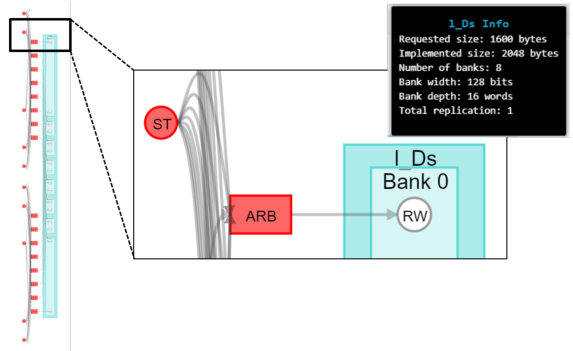
\includegraphics[width=0.7\textwidth]{images/arb}
    \caption{Local memory structure with arbitration units (ARB)}
    \label{fig:arb}
\end{figure}

The kernels were analysed by looking at the synthesized reports and it was noticed that
the 18.1.1 version of the Intel OpenCL compiler, automatically unrolled the loops which were used
to write data into the local memory from constant memory in both the kernels.
The auto-unrolling created parallel store operations which resulted in the
different banking and replication factor of the memories. With different
banking and replication factors, the compiler was not able to optimize
all the memory accesses and produced stallable memory architecture for the
local memories. This was resolved by adding explicitly \texttt{pragma unroll 1} to the
write loops, which prevented the duplication of store operations and
restored the memory architecture as shown in Figure \ref{fig:restored}
\begin{figure}[ht]%
    \centering
    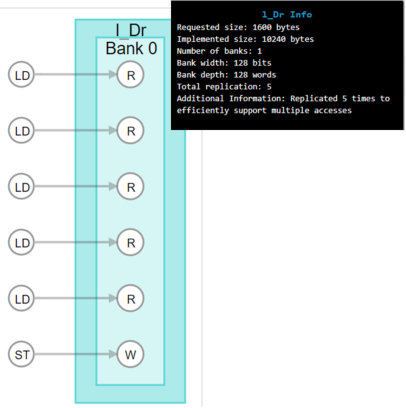
\includegraphics[width=0.45\textwidth]{images/fixed_arb}
    \caption{Local memory structure after addition with pragma unroll 1}
    \label{fig:restored}
\end{figure}


% Kernel pipelining issue